\documentclass[T4paper.tex]{subfiles}

\begin{document}

\begin{figure}
\begin{subfigure}{\textwidth}
   \centering
   \frame{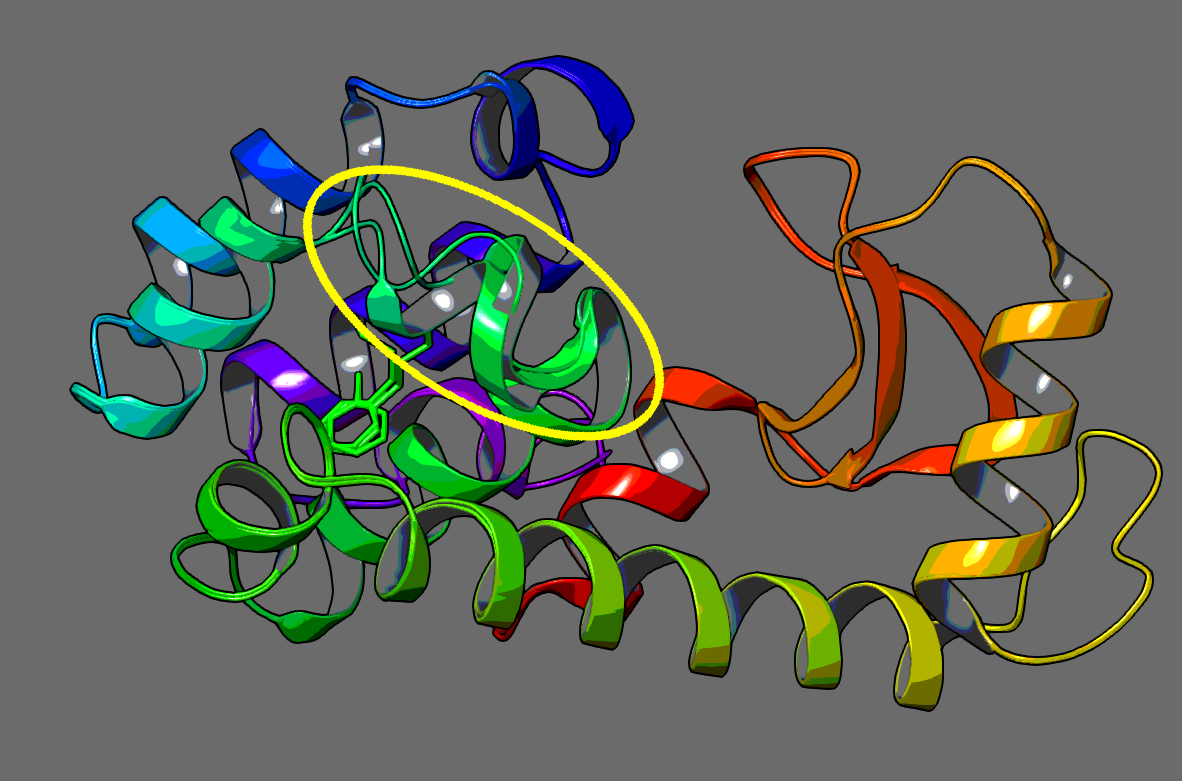
\includegraphics[width=\textwidth]{VMDscripts/Figures/T4_lysozyme_edit.png}}
   \caption{T4-L99A}
   \label{fig:T4-L99A_protein}
\end{subfigure}
\centering
\begin{subfigure}{\textwidth}
  \centering
   \frame{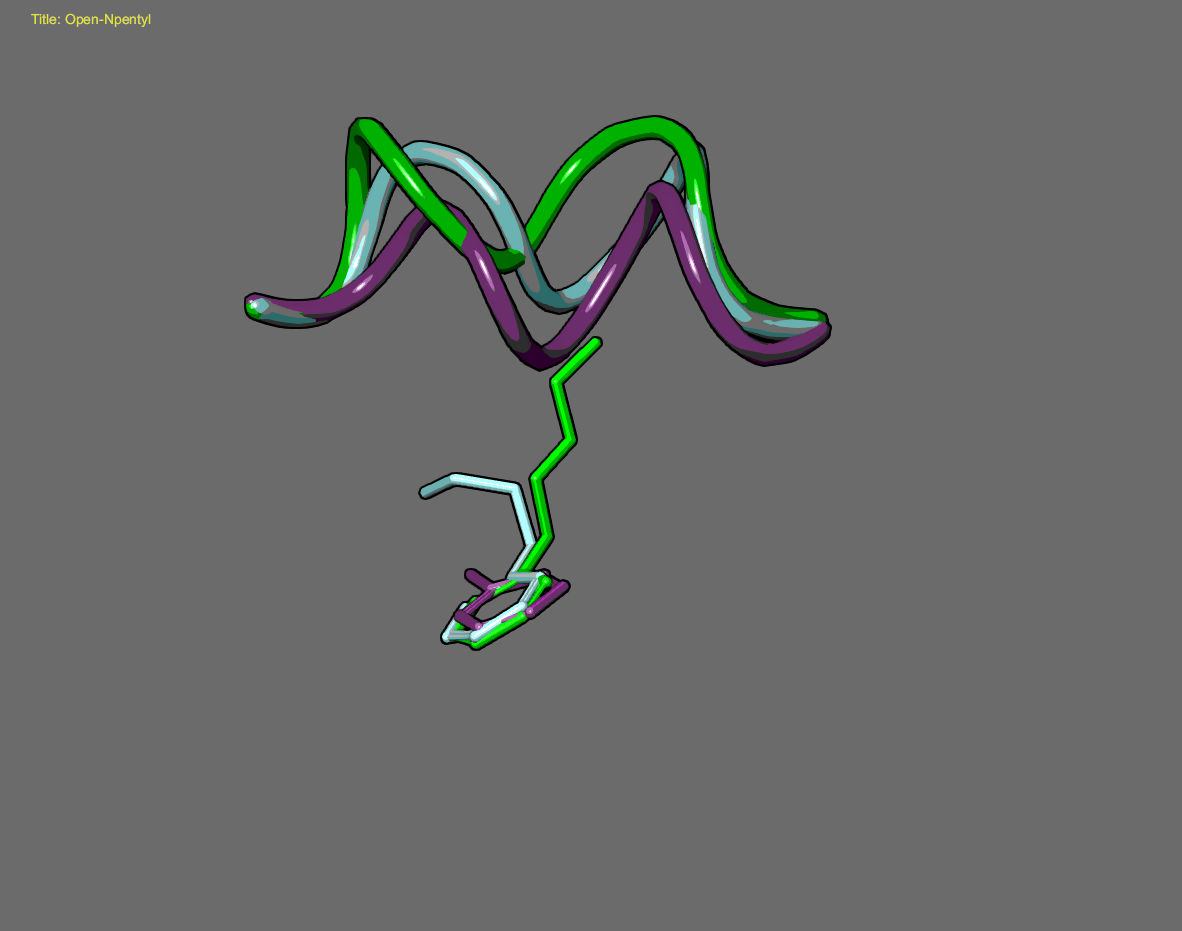
\includegraphics[trim={8cm 8cm 12cm 3cm}, clip, width=\textwidth,height=8cm]{VMDscripts/Figures/ProteinTube.png}}
   \caption{T4-L99A}
   \label{fig:T4-L99A_tube}
\end{subfigure}%
\caption{T4-L99A}
\label{fig:T4-L99A}
\end{figure}

\begin{figure}[!ht]
   \frame{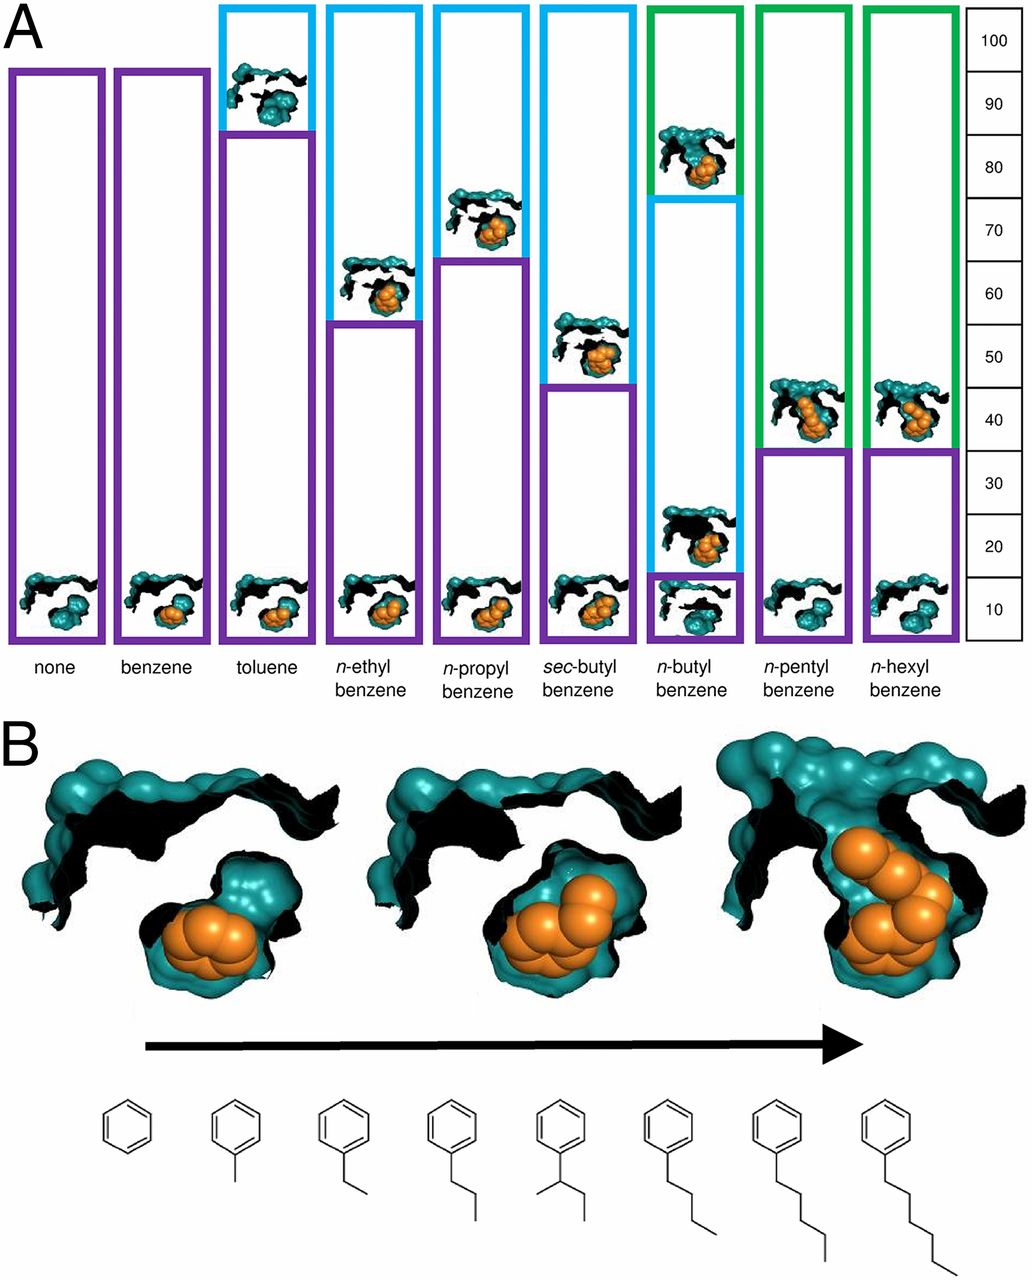
\includegraphics[width=\textwidth]{VMDscripts/Figures/F2large.jpg}}
   \caption{"Congeneric ligands are accommodated in L99A with conformational changes. (A) In the L99A cavity, the ligand poses were assigned to their respective protein conformations by matching the ligand occupancy with that of the F-helix conformation, which was typically unambiguous. (B) Molecular surface of the cavity, cut away to reveal the ligand (orange space-filling model), in examples of the closed (benzene complex), intermediate (ethylbenzene complex), and open (n-hexylbenzene complex) conformations. The full congeneric series is shown."
   Adapted figure\cite{Merski2015}}
   \label{fig:loop-occ}
\end{figure}

\begin{figure}
\begin{subfigure}{\textwidth}
   \centering
   \frame{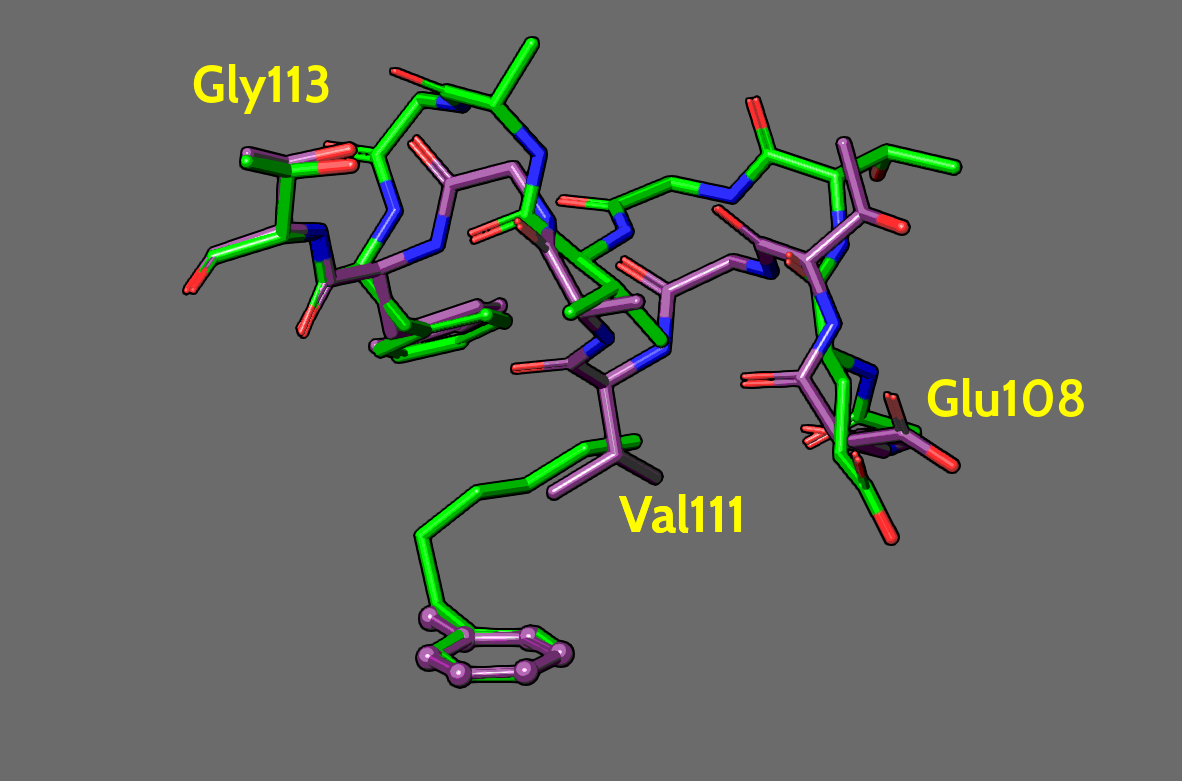
\includegraphics[trim={5cm 2cm 3cm 1cm}, clip, width=\textwidth,height=10cm]{VMDscripts/Figures/C2O.png}}
   \caption{Selected pREST residues}
   \label{fig:C2O}
\end{subfigure}
\centering
\begin{subfigure}{.5\textwidth}
  \centering
   \frame{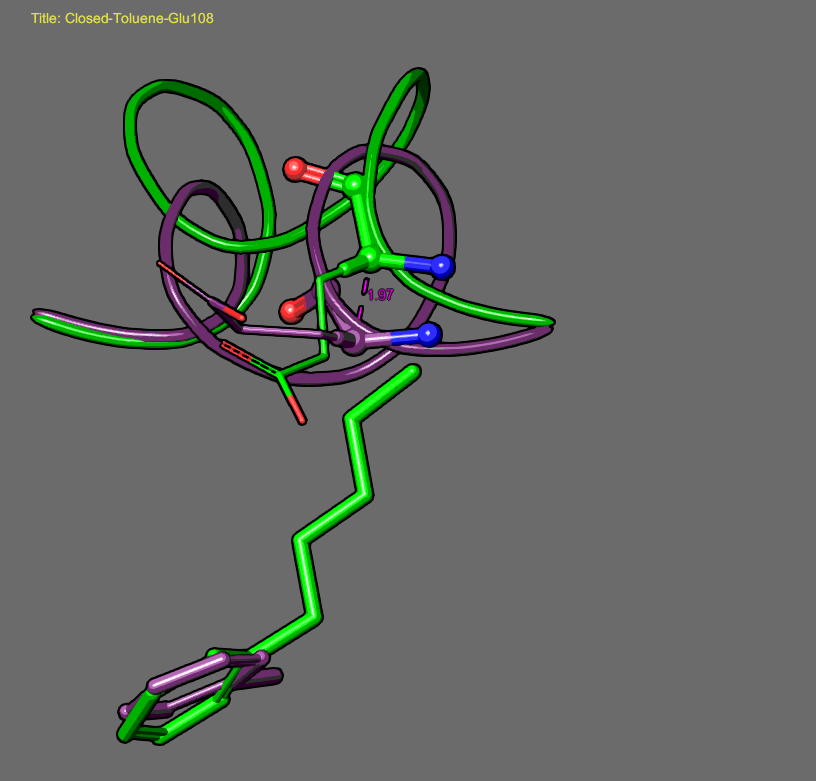
\includegraphics[trim={1cm 1cm 8cm 2cm}, clip, width=\textwidth,height=10cm]{VMDscripts/Figures/Glu108-C2O.png}}
   \caption{Residue Glu108}
   \label{fig:Glu108-C2O}
\end{subfigure}%
\begin{subfigure}{.5\textwidth}
   \centering
   \frame{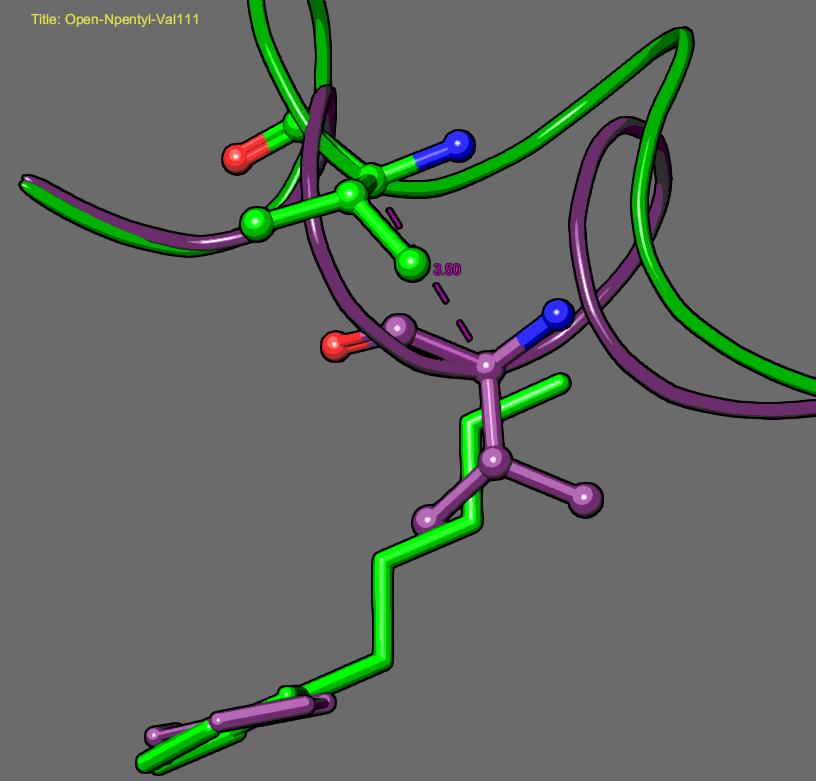
\includegraphics[trim={5cm 0cm 0cm 1cm}, clip, width=\textwidth,height=10cm]{VMDscripts/Figures/Val111-C2O.png}}
   \caption{Residue Val111}
   \label{fig:Val111-C2O}
\end{subfigure}
\caption{pREST residues}
\label{fig:pRESTresidues}
\end{figure}

\begin{figure}
\begin{subfigure}{\textwidth}
   \centering
   \frame{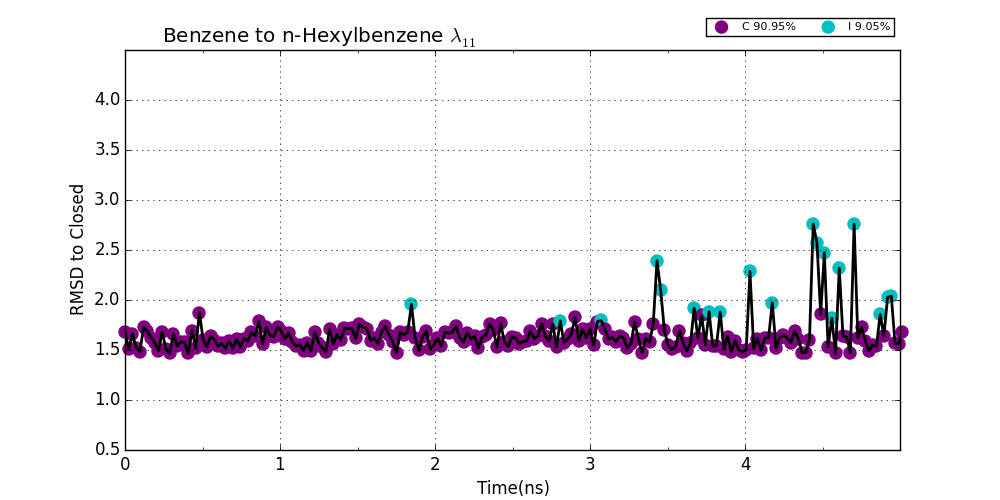
\includegraphics[trim={1.5cm 0 2cm 0.25cm}, clip, width=\textwidth,height=8cm]{VMDscripts/c_opls3_1/plots/0-5ns/RMSD-replica11.png}}
   \caption{Closed - Benzene to n-Hexylbenzene 0-5ns RMSD Replica11}
   \label{fig:c_opls3_1/RMSD-replica11}
\end{subfigure}
\centering
\begin{subfigure}{\textwidth}
  \centering
   \frame{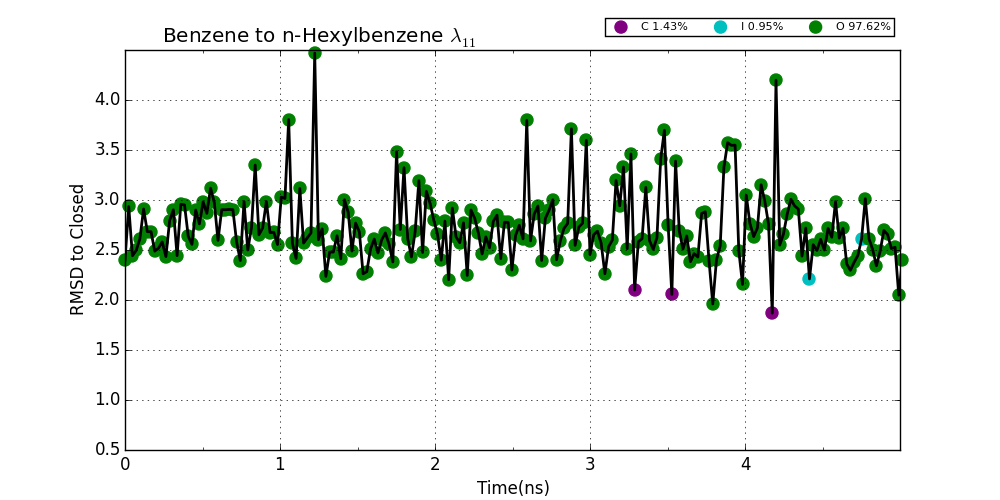
\includegraphics[trim={1.5cm 0 2cm 0.25cm}, clip, width=\textwidth,height=8cm]{VMDscripts/o_opls3_1/plots/0-5ns/RMSD-replica11.png}}
   \caption{Open - Benzene to n-Hexylbenzene 0-5ns RMSD Replica11}
   \label{fig:o_opls3_1/RMSD-replica11}
\end{subfigure}%
\caption{Benzene To n-Hexylbenzene (Default)}
\label{fig:benzene_to_n-hexyl}
\end{figure}

\begin{figure}
\begin{subfigure}{\textwidth}
   \centering
   \frame{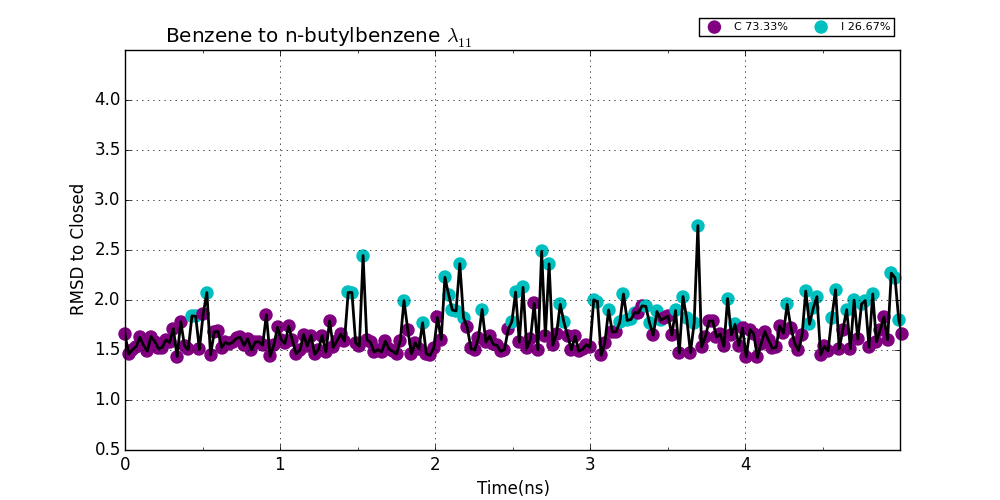
\includegraphics[trim={1.5cm 0 2cm 0.25cm}, clip, width=\textwidth,height=8cm]{VMDscripts/c_exp_opls3_11/plots/0-5ns/RMSD-replica11.png}}
   \caption{Closed - Benzene to n-butylbenzene 0-5ns RMSD Replica11}
   \label{fig:c_exp_opls3_11/RMSD-replica11}
\end{subfigure}
\centering
\begin{subfigure}{\textwidth}
  \centering
   \frame{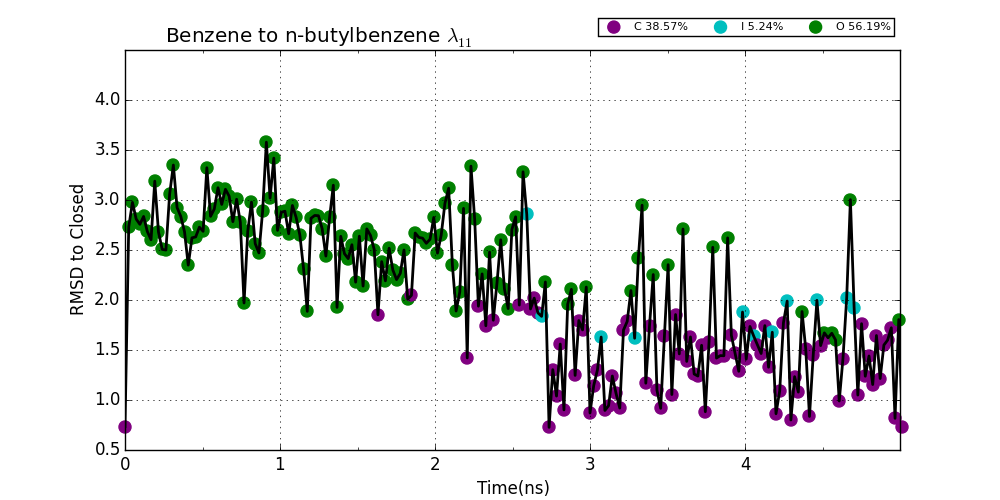
\includegraphics[trim={1.5cm 0 2cm 0.25cm}, clip, width=\textwidth,height=8cm]{VMDscripts/o_exp_opls3_24/plots/0-5ns/RMSD-replica11.png}}
   \caption{Open - Benzene to n-butylbenzene 0-5ns RMSD Replica11}
   \label{fig:o_exp_opls3_24/RMSD-replica11}
\end{subfigure}%
\caption{Benzene To n-Butylbenzenebenzene (Default)}
\label{fig:benzene_to_n-butyl}
\end{figure}


\begin{figure}[!ht]
   \frame{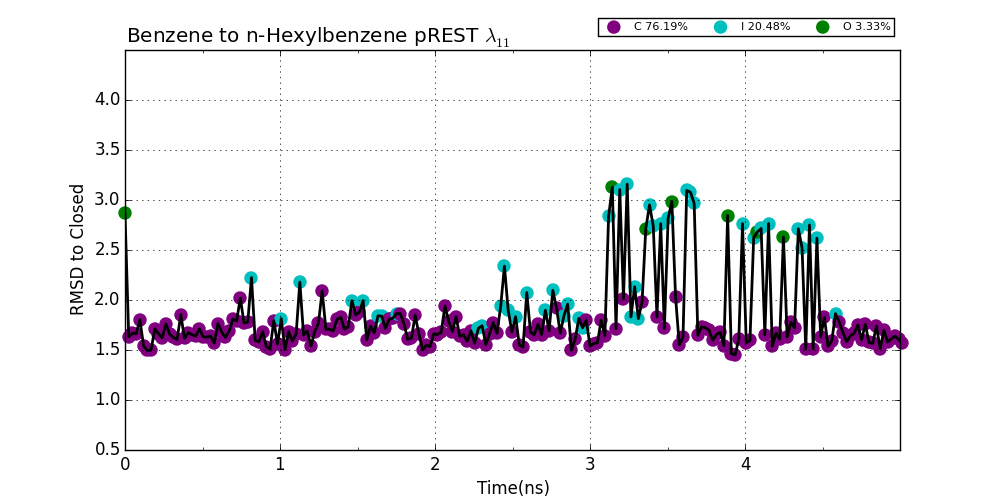
\includegraphics[trim={1.5cm 0 2cm 0.25cm}, clip, width=\textwidth,height=8cm]{VMDscripts/c_opls3_rest1_extend_1e/plots/0-5ns/RMSD-replica11.png}}
   \caption{Closed - Benzene to n-Hexylbenzene 0-5ns RMSD Replica11 pREST}
   \label{fig:c_opls3_rest1_1/RMSD-replica11}
\end{figure}

\begin{figure}[!ht]
   \frame{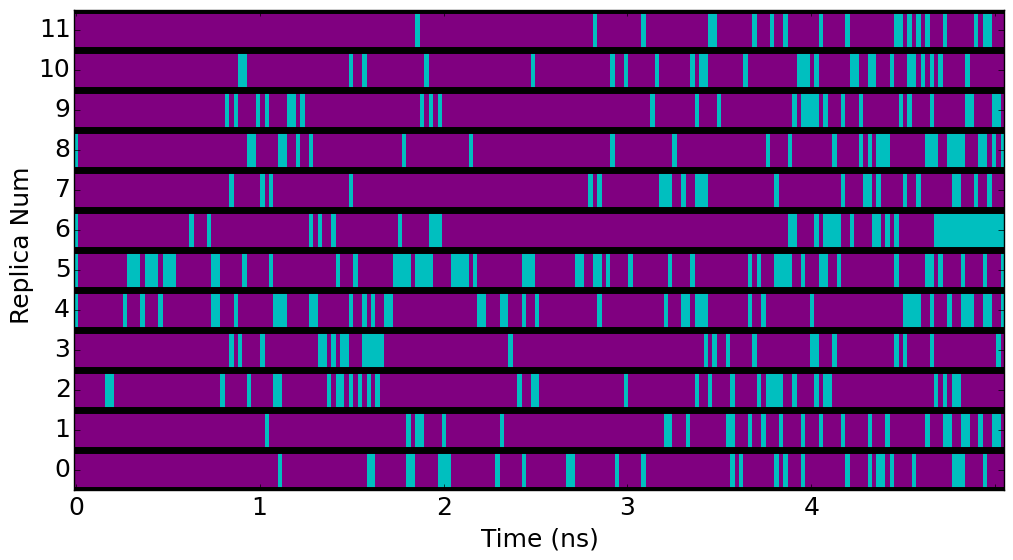
\includegraphics[trim={1.5cm 0 2cm 0.25cm}, clip, width=\textwidth,height=8cm]{VMDscripts/c_opls3_1/plots/colormap/cmap-0-5ns.png}}
   \caption{Closed - Benzene to n-Hexylbenzene 0-5ns Colormap}
   \label{fig:c_opls3_1/colormap}
\end{figure}

\begin{figure}[!ht]
   \frame{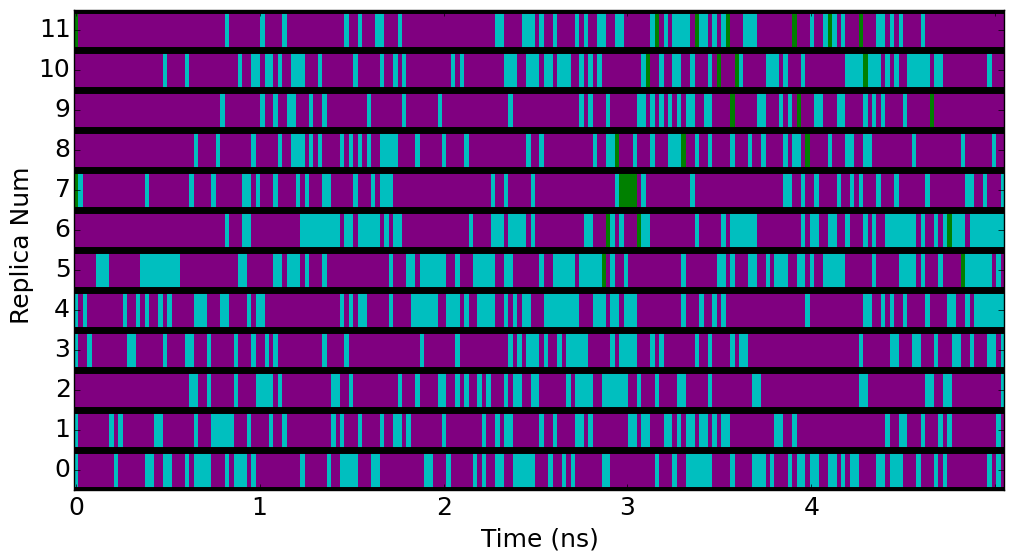
\includegraphics[trim={1.5cm 0 2cm 0.25cm}, clip, width=\textwidth,height=8cm]{VMDscripts/c_opls3_rest1_extend_1e/plots/colormap/cmap-0-5ns.png}}
   \caption{Closed - Benzene to n-Hexylbenzene 0-5ns Colormap pREST}
   \label{fig:c_opls3_rest1_1/colormap}
\end{figure}

\begin{figure}[!ht]
   \frame{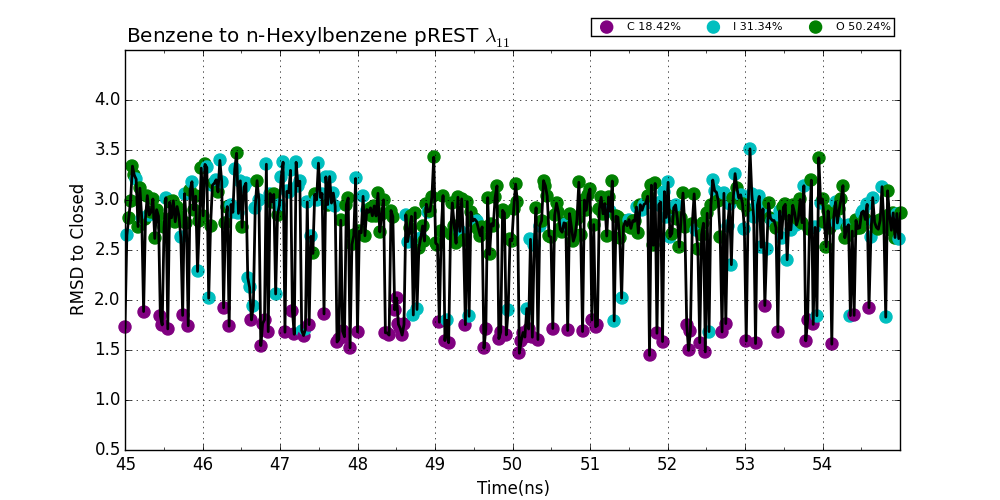
\includegraphics[trim={1.5cm 0 2cm 0.25cm}, clip, width=\textwidth,height=8cm]{VMDscripts/c_opls3_rest1_extend_1e/plots/45-55ns/RMSD-replica11.png}}
   \caption{Closed - Benzene to n-Hexylbenzene 45-55ns RMSD Replica11 pREST}
   \label{fig:c_opls3_rest1_1/45-55ns/RMSD-replica11}
\end{figure}

\begin{figure}[!ht]
   \frame{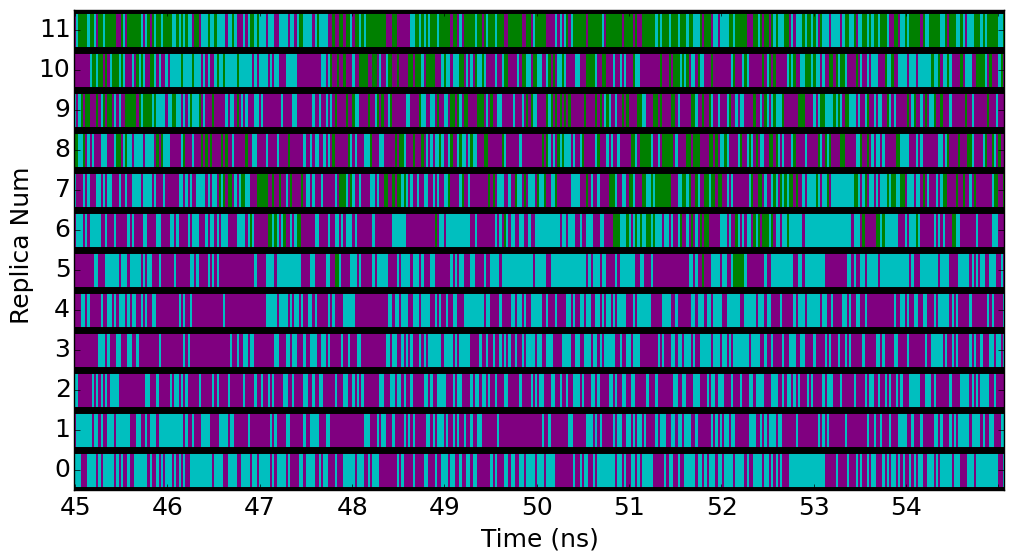
\includegraphics[trim={1.5cm 0 2cm 0.25cm}, clip, width=\textwidth,height=8cm]{VMDscripts/c_opls3_rest1_extend_1e/plots/colormap/cmap-45-55ns.png}}
   \caption{Closed - Benzene to n-Hexylbenzene 45-55ns Colormap pREST}
   \label{fig:c_opls3_rest1_1/cmap-45-55ns}
\end{figure}

\begin{figure}
\centering
\begin{subfigure}{.5\textwidth}
  \centering
   \frame{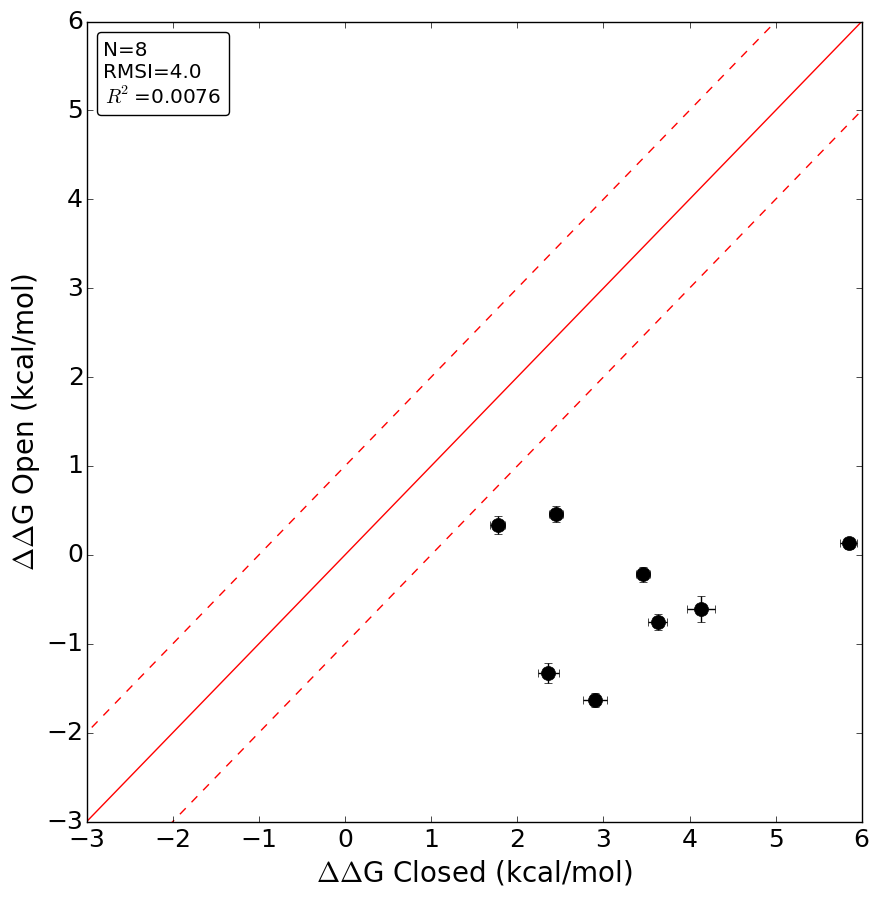
\includegraphics[width=\textwidth,height=10cm]{VMDscripts/XYplot/C2O_xyplot.png}}
   \caption{Closed-Open XYplot (Default)}
   \label{fig:C2O_xyplot}
\end{subfigure}%
\begin{subfigure}{.5\textwidth}
   \centering
   \frame{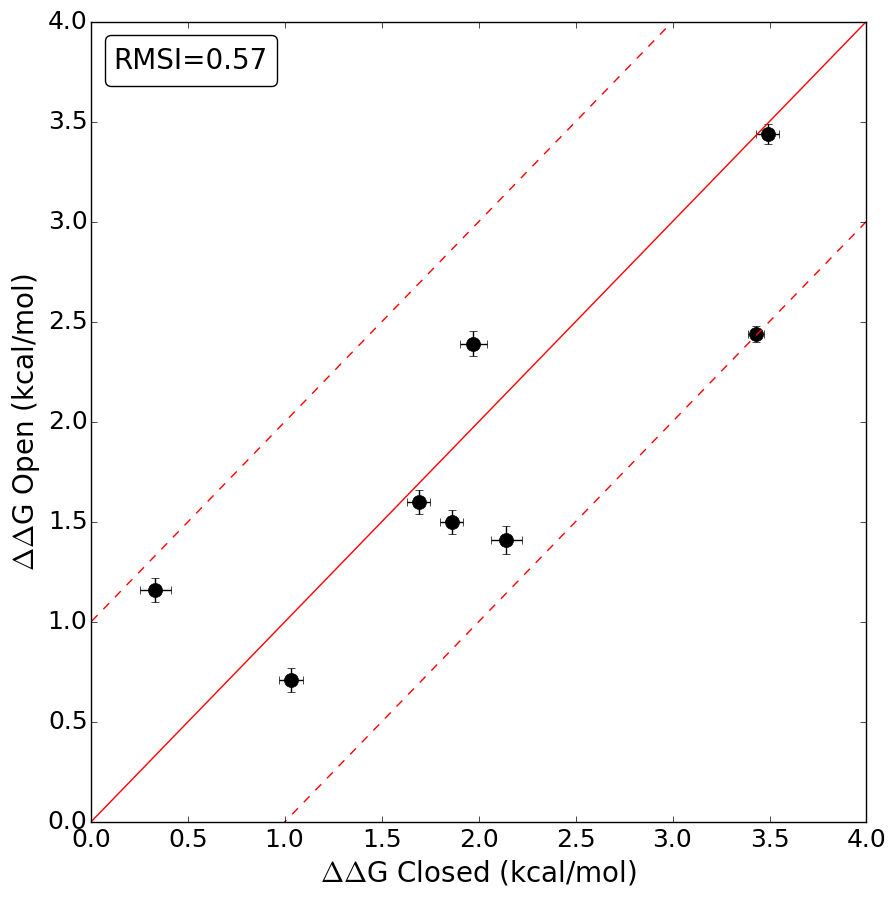
\includegraphics[width=\textwidth,height=10cm]{VMDscripts/XYplot/C2O_pREST_xyplot.png}}
   \caption{Closed-Open XYplot (pREST)}
   \label{fig:C2O_xyplot_pREST}
\end{subfigure}
\caption{Closed-Open}
\label{fig:C2O_xy}
\end{figure}

\begin{figure}
\centering
\begin{subfigure}{.5\textwidth}
  \centering
   \frame{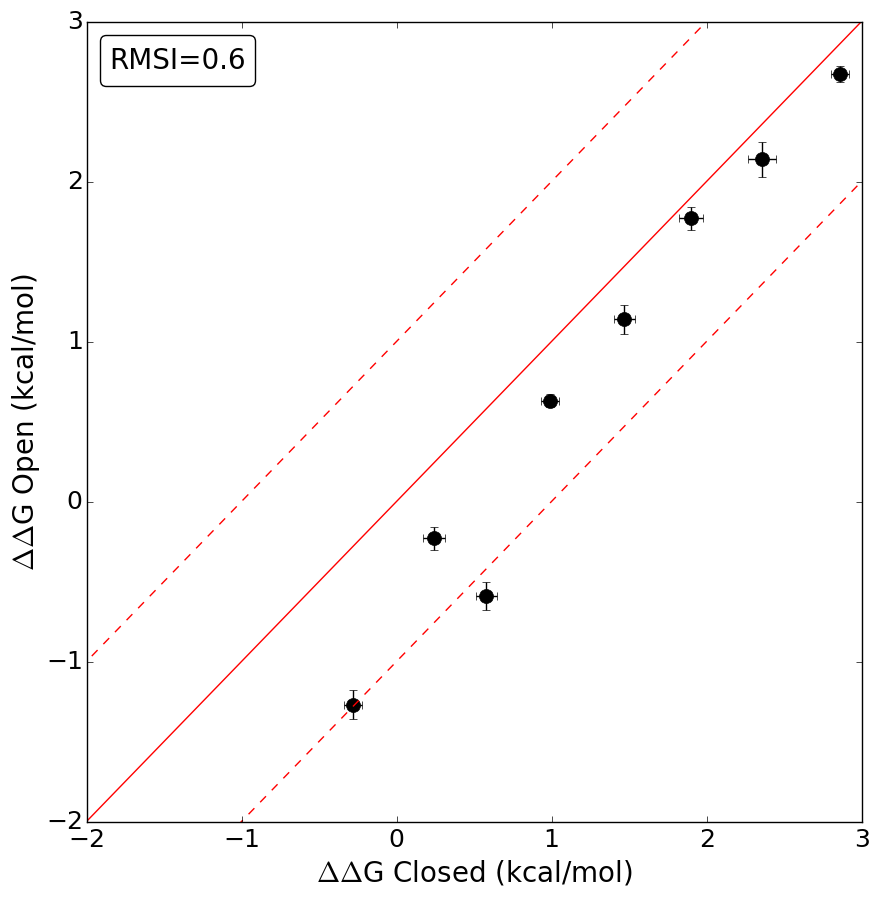
\includegraphics[width=\textwidth,height=10cm]{VMDscripts/XYplot/C2I_xyplot.png}}
   \caption{Closed-Int XYplot (Default)}
   \label{fig:C2I_xyplot}
\end{subfigure}%
\begin{subfigure}{.5\textwidth}
   \centering
   \frame{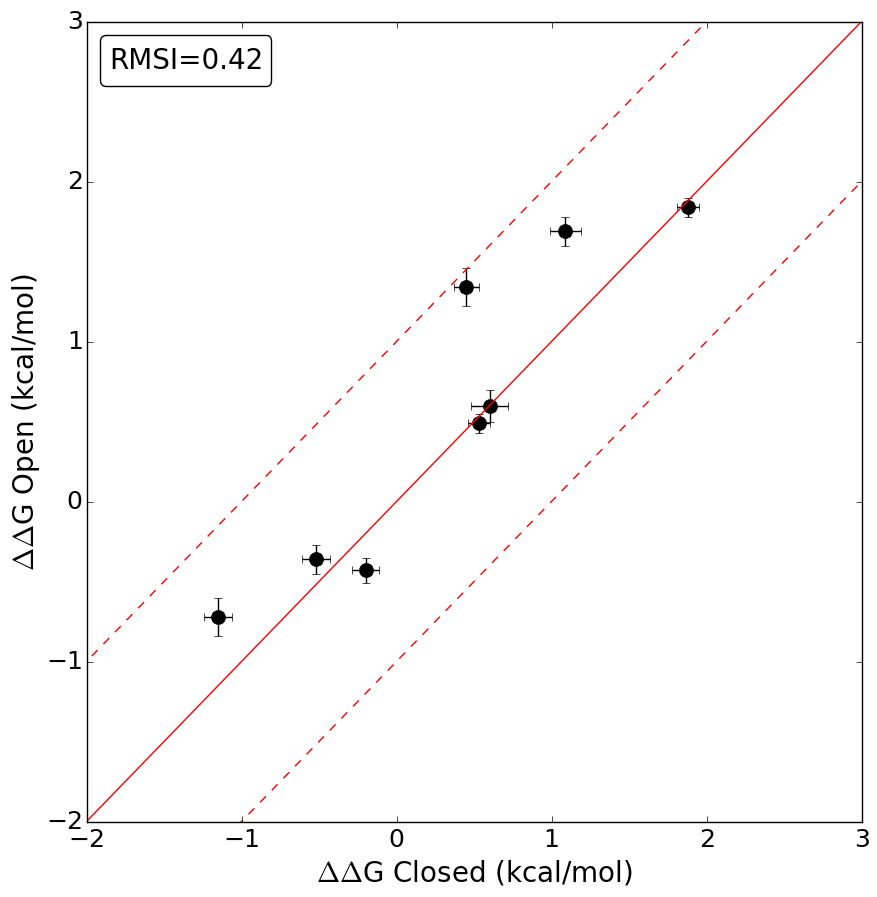
\includegraphics[width=\textwidth,height=10cm]{VMDscripts/XYplot/C2I_pREST_xyplot.png}}
   \caption{Closed-Int XYplot (pREST)}
   \label{fig:C2I_xyplot_pREST}
\end{subfigure}
\caption{Closed-Int}
\label{fig:C2I_xy}
\end{figure}

\begin{figure}
\centering
\begin{subfigure}{.5\textwidth}
  \centering
   \frame{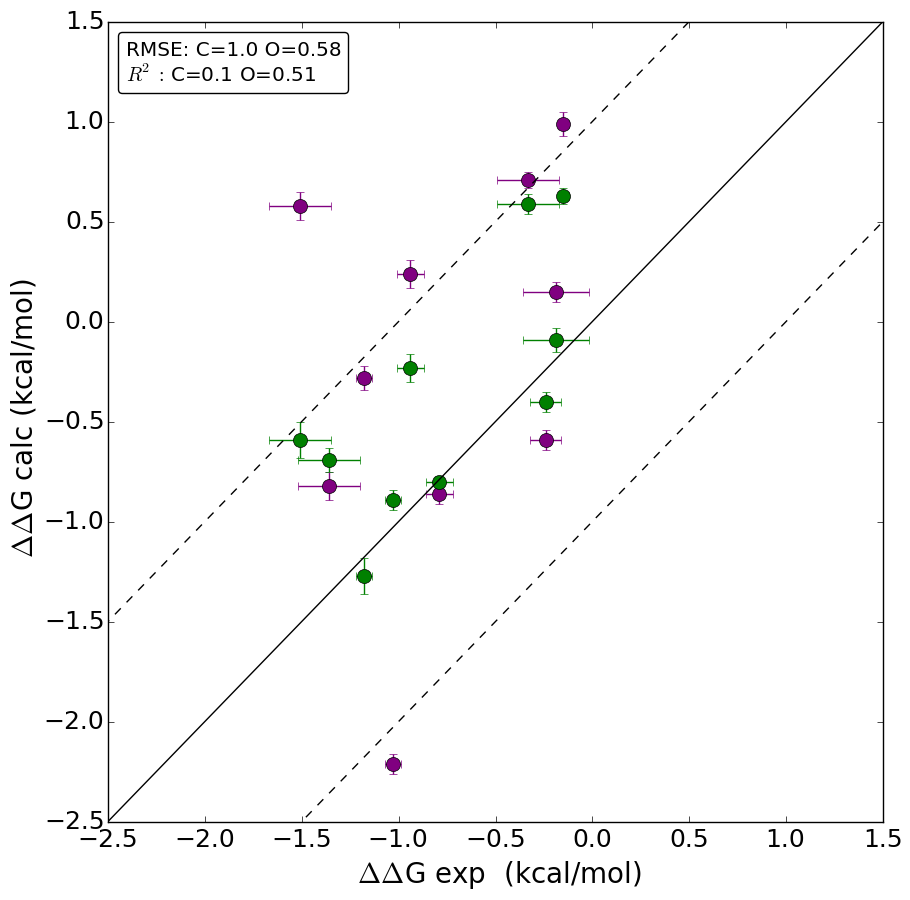
\includegraphics[width=\textwidth,height=10cm]{VMDscripts/XYplot/exp_xyplot.png}}
   \caption{Exp XYplot (Default)}
   \label{fig:exp_xyplot}
\end{subfigure}%
\begin{subfigure}{.5\textwidth}
   \centering
   \frame{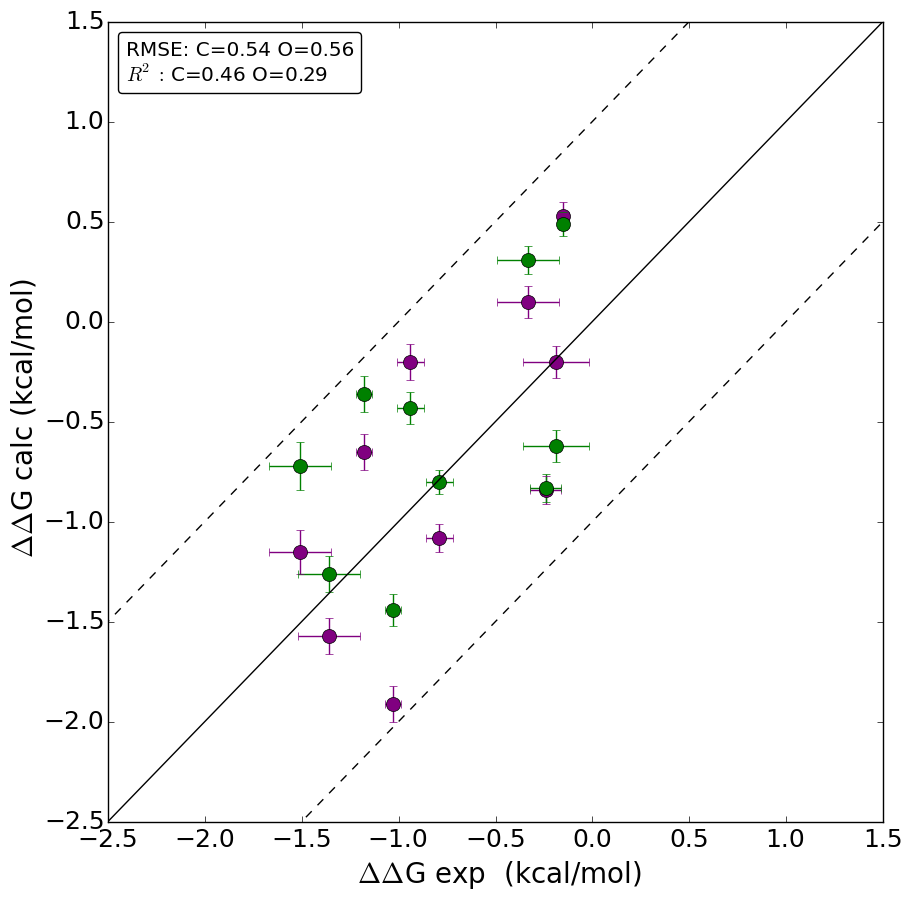
\includegraphics[width=\textwidth,height=10cm]{VMDscripts/XYplot/exp_pREST_xyplot.png}}
   \caption{Closed-Int XYplot (pREST)}
   \label{fig:exp_xyplot_pREST}
\end{subfigure}
\caption{Closed-Exp}
\label{fig:exp_xy}
\end{figure}

\end{document}